\section{2D-LiDARとYOLOv5を用いた手法}
飯田一成らのプロジェクト\cite{深層学習を用いた人追従機能の開発}では、
リアルタイム物体検出アルゴリズムであるYOLOv5を用いて、2D-LiDARの距離データから
人の脚部を検出している。\\ \indent
提案手法は、Fig. \ref{2-1_Image of centroid}のように2D-LiDARの距離データを画像化し、学習したYOLOv5の物体検出により画像から
人の脚部を検出する。複数検出する場合があるため、検出する範囲を一定の位置に設定している。
また、衝突回避機能を実装することで、安全性を考慮した人追従機能を提案している。\\ \indent
実験方法は、追従実験と衝突回避実験がある。追従実験ではFig. \ref{2-1_Data Acquisition Environment} 3つの経路を設定し、1回のみの試行である。
衝突回避実験では、人追従中に追従対象者とロボットとの間に障害物を設置し、停止したかを
3つの状況に分けてそれぞれ10回試行している。実験結果は、追従実験では3つの経路において20[m]
の人追従ができていたが、雑多な環境下では追従中に停止することがあった。
衝突回避実験ではTable \ref{2-1_Success rate of emergency stops on each road}
に示すように、すべての試行において衝突回避ができていた。

\begin{figure*}[h]
  \begin{center}
  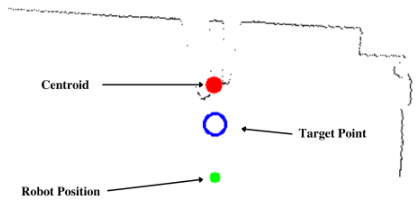
\includegraphics[height=60mm,clip]{figure/2-1_Image-of-centroid.png}
  \caption{Image of centroid\cite{深層学習を用いた人追従機能の開発}}
  \label{2-1_Image of centroid}
  \end{center}
\end{figure*}

\begin{figure*}[h]
  \begin{center}
  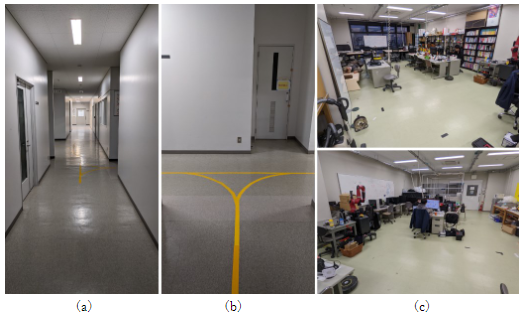
\includegraphics[height=80mm,clip]{figure/2-1_Data-Acquisition-Environment.png}
  \caption{Data Acquisition Environment\cite{深層学習を用いた人追従機能の開発}}
  \label{2-1_Data Acquisition Environment}
  \end{center}
\end{figure*}

\begin{table}[h]
  \begin{center}
    \caption{{Success rate of emergency stops on each road\cite{深層学習を用いた人追従機能の開発}}
    \label{2-1_Success rate of emergency stops on each road}}
    \scalebox{1.0}[0.9]{
      \begin{tabular}{c|ccc} \hline
        \multicolumn{1}{c|}{} & \multicolumn{3}{c}{Distance between robot and obstacle} \\
        \cline{2-4}
        \multicolumn{1}{c|}{}
          & 0.1[m] & 0.2[m] & 0.3[m] \\ \hline
          Straight road & 100[\%] & 100[\%] & 100[\%] \\
          Curved road & 100[\%] & 100[\%] & 100[\%] \\
          Miscellaneous road & 100[\%] & 100[\%] & 100[\%] \\ \hline
      \end{tabular}
    }
  \end{center}
\end{table}

\clearpage

\section{2D-LiDARの距離データをクラスタリングする手法}
Fei Luoらの研究\cite{Temporal convolutional networks for multi-person activity recognition using a 2D LIDAR}
では、キッチン内を想定し、人が歩行した軌跡のクラスタリングを行っている。\\ \indent
提案手法は、Fig. \ref{2-2_LIDAR data processing}が処理の全体像である。Fig. \ref{2-2_LIDAR data processing}
(a)では、2D-LiDARから提供される距離データをプロットしている。Fig. \ref{2-2_LIDAR data processing}(b)
では、密度ベースのクラスタリングアルゴリズムである
DBSCAN (Density-Based Spatial Clustering of Applications with Noise)
を用いて距離データをクラスタリングする。\ref{2-2_LIDAR data processing}(c)では、
Fig. \ref{2-2_Human recognition}のように定義した幾何学的特徴をもとにランダムフォレストにより、
人間と非人間の2つに分類する。Fig. \ref{2-2_LIDAR data processing}(c)では、カルマンフィルタを用いて
人間が移動した軌跡を生成し、ガウスノイズなどの軌跡拡張が行われ、
LSTM (Long Short-Term Memory)とTCN (Temporal Convolutional Network)の両方に入力される。
活動クラスに分類される。LSTMは、時間経過に伴って変化するデータを学習できる
RNN(Recurrent Neural Network)の勾配消失問題を解消したものであり、TCNは時系列データに対して
CNN (Convolutional Neural Network)を用いているものである。\\ \indent
実験方法は、学習したLSTMとTCNを用いて、Fig. \ref{2-2_Kitchen scenario}のような環境において
15種類の歩行パターンを分類させ、LSTMとTCNの分類精度の評価を行う。
実験結果はTable \ref{2-2_THE EFFECT OF TRAJECTORY AUGMENTATION}のようになっており、
LSTMよりTCNのほうが分類精度が高いことが明らかになっている。

\begin{figure*}[h]
  \begin{center}
  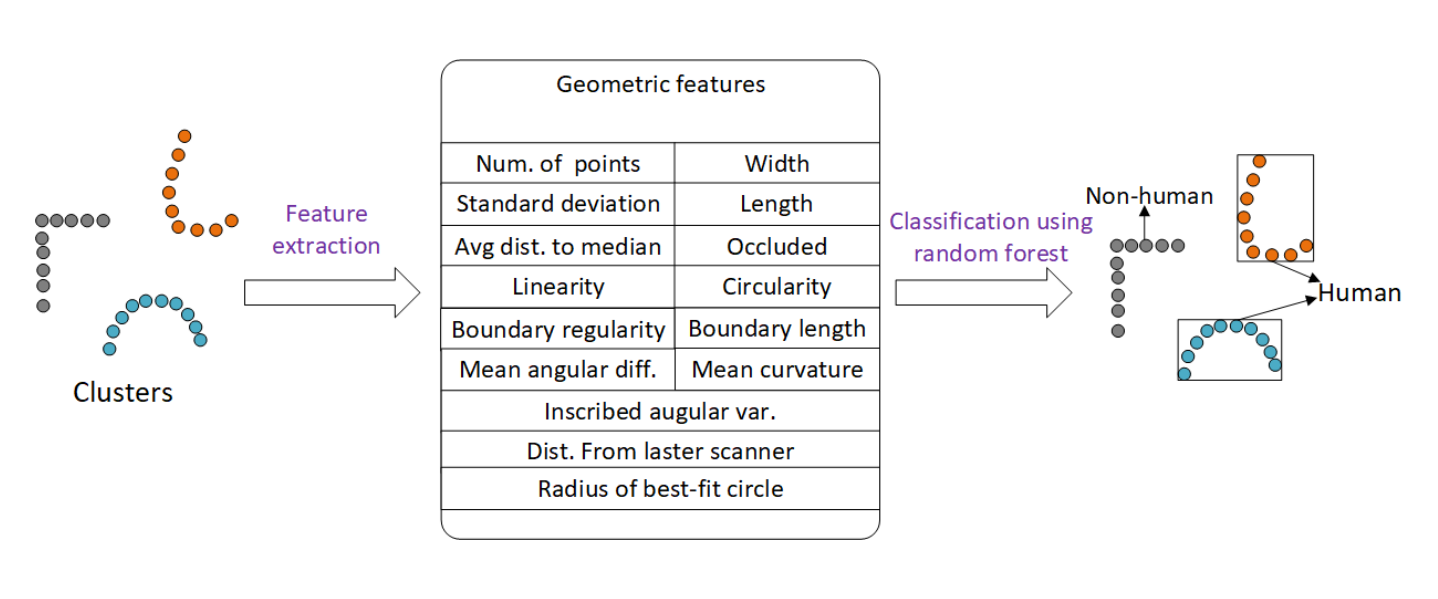
\includegraphics[height=70mm,clip]{figure/2-2_Human-recognition.png}
  \caption{Human recognition\cite{Temporal convolutional networks for multi-person activity recognition using a 2D LIDAR}}
  \label{2-2_Human recognition}
  \end{center}
\end{figure*}

\begin{figure*}[t]
  \begin{center}
  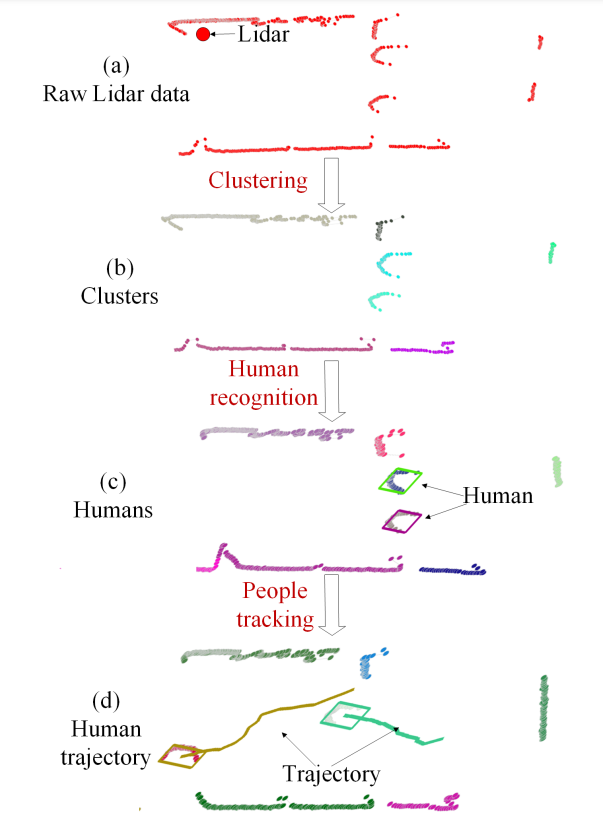
\includegraphics[height=100mm,clip]{figure/2-2_LIDAR-data-processing.png}
  \caption{LIDAR data processing\cite{Temporal convolutional networks for multi-person activity recognition using a 2D LIDAR}}
  \label{2-2_LIDAR data processing}
  \end{center}
\end{figure*}

\begin{figure*}[t]
  \begin{center}
  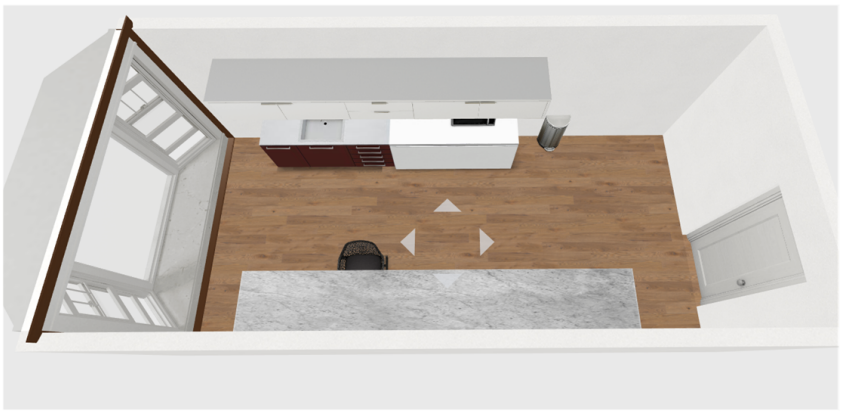
\includegraphics[height=50mm,clip]{figure/2-2_Kitchen-scenario.png}
  \caption{Kitchen scenario\cite{Temporal convolutional networks for multi-person activity recognition using a 2D LIDAR}}
  \label{2-2_Kitchen scenario}
  \end{center}
\end{figure*}

\begin{table}[b]
  \begin{center}
    \caption{{THE EFFECT OF TRAJECTORY AUGMENTATION\cite{Temporal convolutional networks for multi-person activity recognition using a 2D LIDAR}}
    \label{2-2_THE EFFECT OF TRAJECTORY AUGMENTATION}}
    \scalebox{1.0}[0.9]{
      \begin{tabular}{l|c|c|c} \hline
        & OA & Recall & F1 \\ \hline
        TCN with trajectory augmentation & 99.49\% & 99.53\% & 99.51\% \\ \hline
        TCN without trajectory augmentation & 97.96\% & 97.93\% & 97.96\% \\ \hline
        LSTM with trajectory augmentation & 99.39\% & 99.41\% & 99.39\% \\ \hline
        LSTM without trajectory augmentation & 97.65\% & 97.79\% & 97.65\% \\ \hline
      \end{tabular}
    }
  \end{center}
\end{table}

\clearpage

\section{FCNと2D-LiDARを用いた手法}
Ángel Manuel Guerrero-Higuerasらの研究
\cite{Tracking People in a Mobile Robot From 2D LIDAR Scans Using Full Convolutional Neural Networks for Security in Cluttered Environments}
では、FCN(Full Convolutional Neural Networks)を用いて、2D-LiDARの距離データ
から人の両脚部分を検出することで人追従する「PeTra」を提案している。\\ \indent
提案手法は、2D-LiDARからの距離データを画像化し、
Fig. \ref{2-4_cnn}に示すアーキテクチャにより、人の両脚部分をセグメンテーション
することにより、追従対象者を検出している。\\ \indent
実験方法は、Fig. \ref{2-4_env}の左のような環境において、Location1、Location2、Location3
で行われる。また、Fig. \ref{2-4_env}の右にあるタグを追従対象者が所持することにより、
タグの位置を真値としている。PeTraの比較対象として、ROS(Robot Operationg System)が
提供しているLD(Leg Detector)を用いており、追従対象者が所持しているタグからの平均誤差と
標準偏差[m]をPeTraとLDで比較する。
実験結果を、Fig. \ref{2-4_result}とTable \ref{2-4_result_table}に示す。
Fig. \ref{2-4_result}の黄色のマーカーは2D-LiDARの距離データであり、
赤矢印はロボットの位置と向きであり、矢印の先がロボットの位置である。
Fig. \ref{2-4_result}の左が2D-LiDARの距離データのみの画像であり、
中央はPeTraによる推定結果が加えられた画像で、緑色のマーカーは人の中心、
青色のマーカーは脚の位置を示している。
右はLDによる推定結果が加えられた画像である。赤いマーカーは脚の位置を示している。
Fig. \ref{2-4_result}から、LDよりPeTraの方が脚のペアを正しく推定していることが分かる。
また、Table \ref{2-4_result_table}はLocation1、Location2、Location3における、
PeTraとLDの追従対象者が所持しているタグからの平均誤差と標準偏差である。
Table \ref{2-4_result_table}から、LDよりPeTraの方が誤差が50\%少ないことが分かる。
以上のことから、LDより精度が高い人追従ツールを実現していることが分かる。

\begin{figure*}[h]
  \begin{center}
  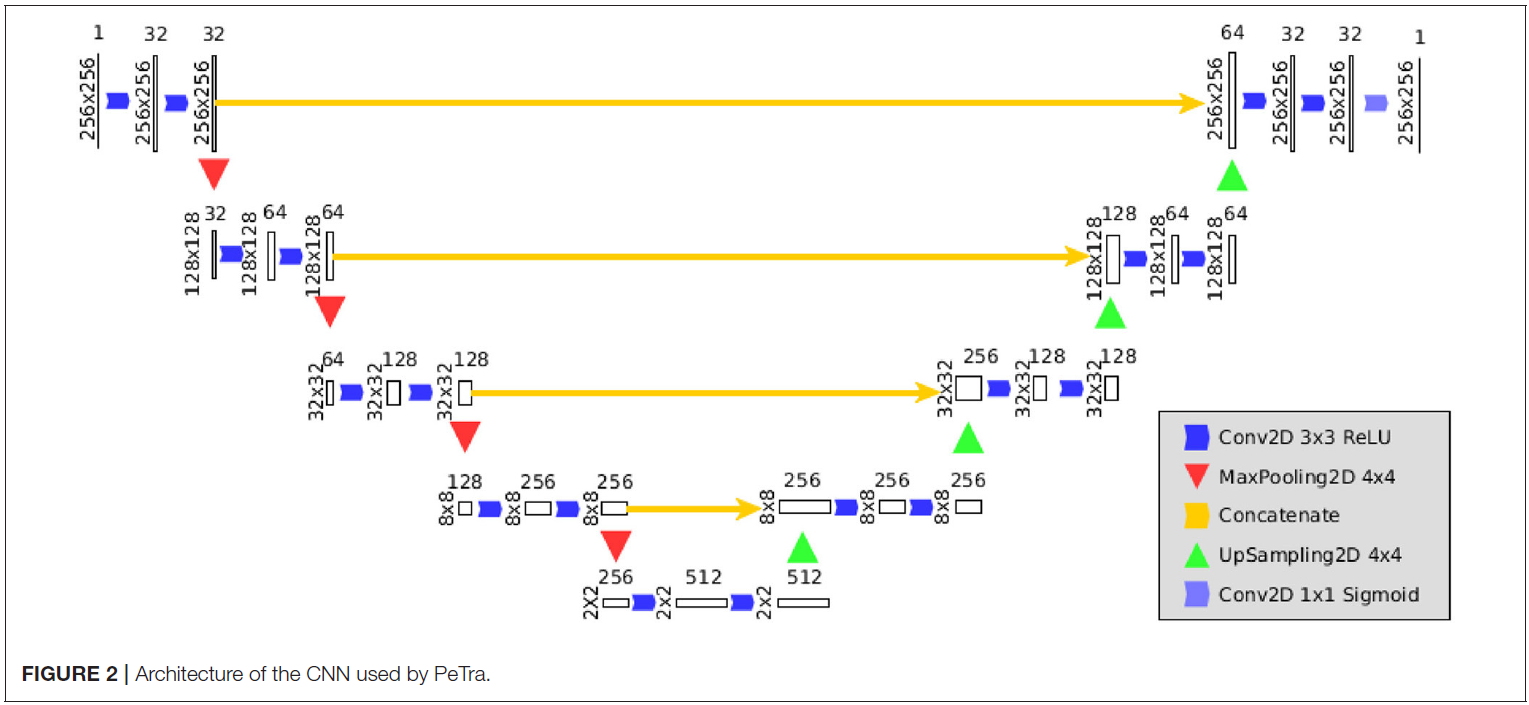
\includegraphics[height=70mm,clip]{figure/2-4_cnn.png}
  \caption{Architecture of the CNN used by PeTra
  \cite{Tracking People in a Mobile Robot From 2D LIDAR Scans Using Full Convolutional Neural Networks for Security in Cluttered Environments}}
  \label{2-4_cnn}
  \end{center}
\end{figure*}

\begin{figure*}[h]
  \begin{center}
  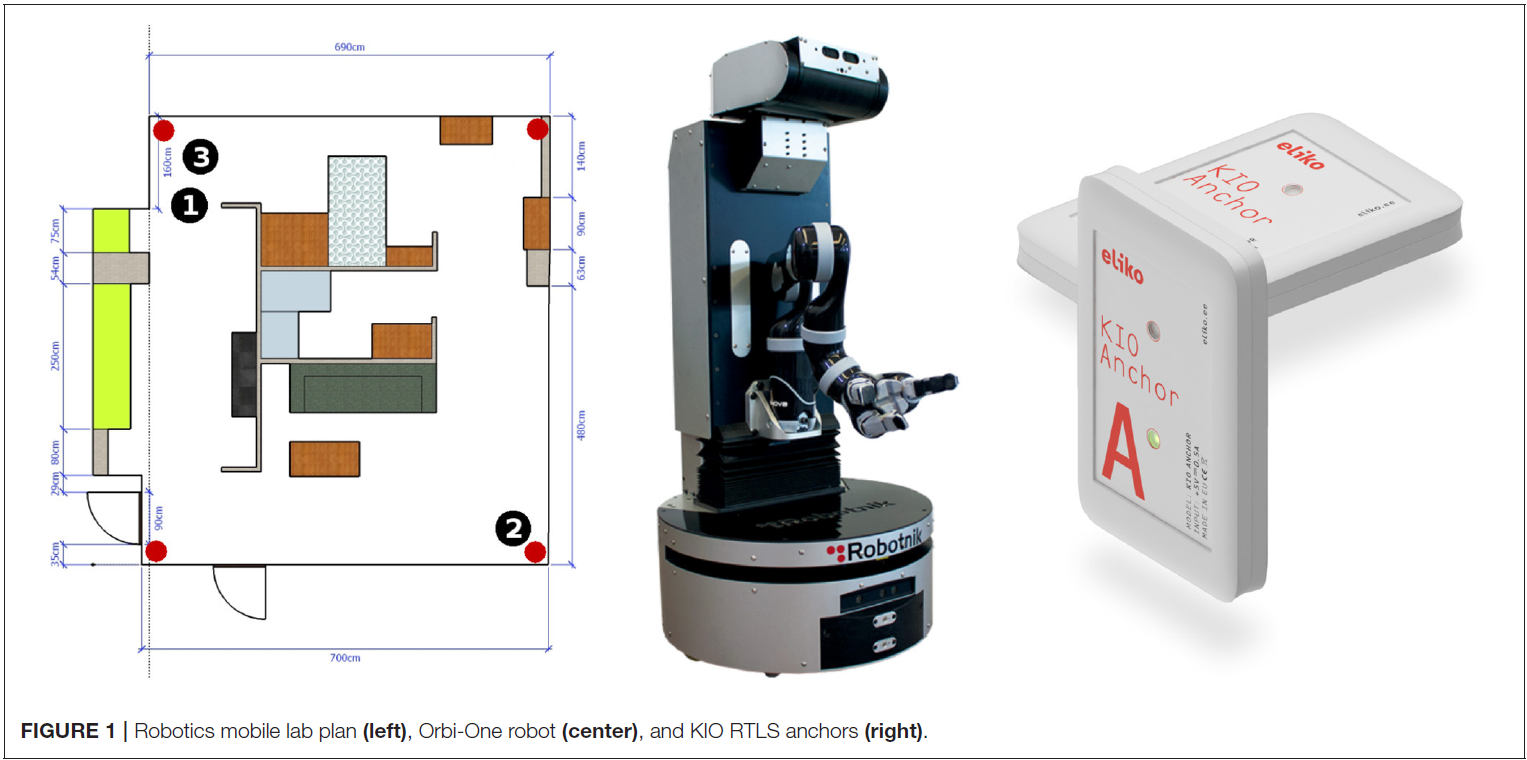
\includegraphics[height=60mm,clip]{figure/2-4_env.png}
  \caption{Robotics mobile lab plan (left), Orbi-One robot (center), and KIO RTLS anchors (right).
  \cite{Tracking People in a Mobile Robot From 2D LIDAR Scans Using Full Convolutional Neural Networks for Security in Cluttered Environments}}
  \label{2-4_env}
  \end{center}
\end{figure*}

\begin{figure*}[h]
  \begin{center}
  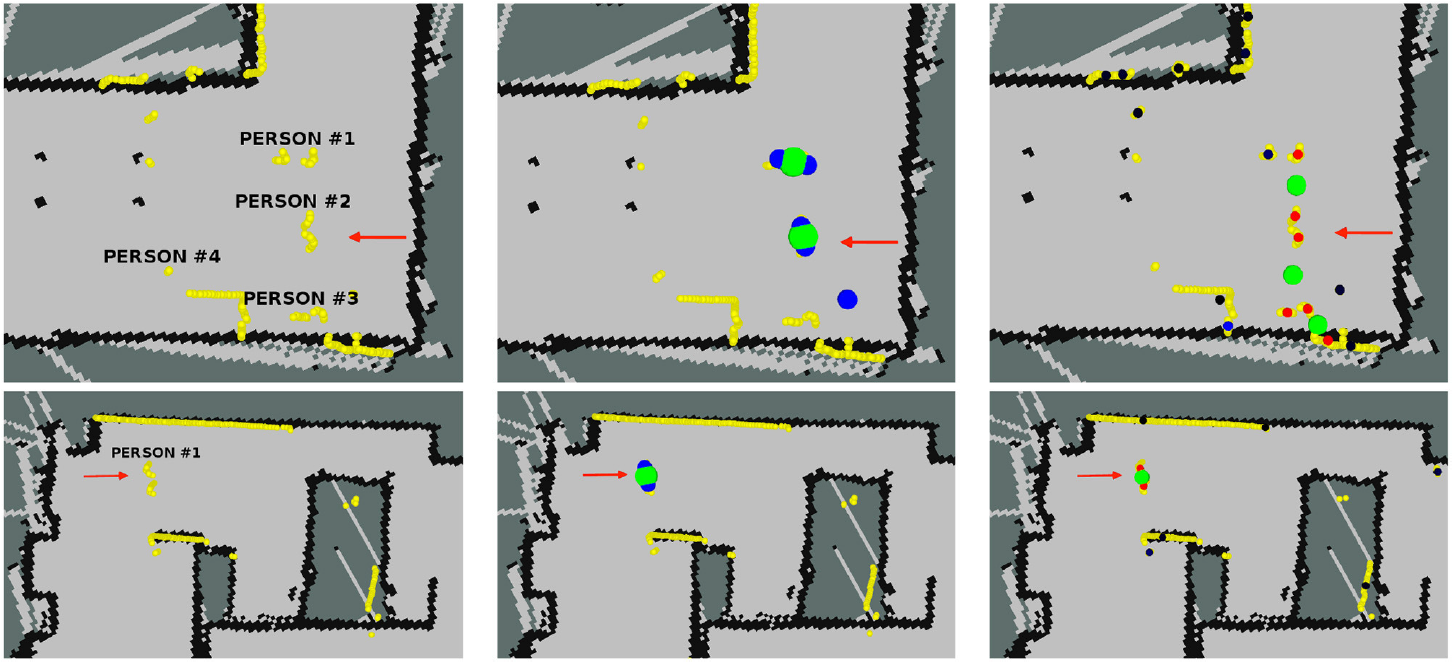
\includegraphics[height=60mm,clip]{figure/2-4_result.png}
  \caption{Comparison image of PeTra and LD by Rviz
  \cite{Tracking People in a Mobile Robot From 2D LIDAR Scans Using Full Convolutional Neural Networks for Security in Cluttered Environments}}
  \label{2-4_result}
  \end{center}
\end{figure*}

\begin{table}[h]
  \begin{center}
    \caption{{Mean error and standard deviation[m] at each location
    \cite{Tracking People in a Mobile Robot From 2D LIDAR Scans Using Full Convolutional Neural Networks for Security in Cluttered Environments}}
    \label{2-4_result_table}}
    \scalebox{1.0}[0.9]{
      \begin{tabular}{c|c|c|c} \hline
        Method & Location 1 & Location 2 & Location3 \\ \hline
        PeTra & $0.17 (\pm0.13)$ & $0.43 (\pm0.22)$ & $0.20 (\pm0.13)$ \\
        LD & $0.30 (\pm0.15)$ & $0.75 (\pm0.28)$ & $0.49 (\pm0.33)$ \\ \hline
      \end{tabular}
    }
  \end{center}
\end{table}

\clearpage

\section{AOAタグと2D-LiDARを組み合わせた手法}
DAPING JINらの研究\cite{A Robust Autonomous Following Method for Mobile Robots in Dynamic Environments}
では、Fig. \ref{2-3_real}のような環境を想定し、AOAタグと2D-LiDARのデータから人を検出している。\\ \indent
提案手法は、システム全体はFig. \ref{2-3_system}のようになっており、2D-LiDARとAOAタグの
データをカルマンフィルタを用いた追跡情報を統合することで人の位置を正確に追跡している。
ロボットの制御では、Dynamic Window Approachを改良したFMM-DWAを用いて
障害物に衝突しないロボット制御を実装している。
AOAタグは、位置情報を送信するデバイスであり、人にAOAタグを所持してもらい、ロボットが位置情報
を受信している。Fig. \ref{2-3_aoa}は、AOAタグとカルマンフィルタの追従軌跡を比較した
ものであり、赤いデータがAOAタグ、黒いデータがカルマンフィルタのデータである。
AOAタグはカルマンフィルタの追跡軌跡よりノイズが多いことがわかる。
また、2D-LiDARによる人の脚部検出では、2D-LiDARのデータをクラスタリングし、
各クラスタに対して、2D-LiDARのデータ数や幅と長さなどの幾何学的特徴が生成され、
幾何学的特徴に基づいて、Fig. \ref{2-3_overview}のように人の脚かその他に分類する。
Fig. \ref{2-3_laser}は、2D-LiDARとカルマンフィルタの追跡軌跡を比較したものであり、
赤いデータが2D-LiDAR、黒いデータがカルマンフィルタのデータである。
カルマンフィルタより2D-LiDARの追跡軌跡の方が滑らかであると述べられている。
これらのAOAタグと2D-LiDARの追跡軌跡を組み合わせたものがFig. \ref{2-3_aoaANDlaser}
である。緑色の軌跡がAOAタグ、赤い軌跡は2D-LiDAR、黒い軌跡はカルマンフィルタの軌跡である。
2D-LiDARでの追従は、Fig. \ref{2-3_aoaANDlaser}の「Laser Tracking Failure」部分
で追従ができなくなった。しかし、「Laser Tracking Recovery」の部分で再び追従対象を発見
し追従を再開した。
実験方法は、Fig. \ref{2-3_real}のような障害物がいくつかある環境において、
モデル予測制御であるMPEPCとFMM-DWAによるロボット制御の比較である。
実験結果をTable \ref{2-3_result_table}に示す。
ロボット台車の加速度では、FMM-DWAにおける加速度が$1m/s^2$未満である場合が90\%以上であり、
MPEPCにおける加速度が$1m/s^2$未満である場合が68\%であった。
また、ロボット台車の旋回半径がMPEPCでは、1mより小さい制御コマンドは全体の8\%であり、
FMM-DWAの2.6倍である。
さらに、人の軌道とロボットの軌道の追跡率は、FMM-DWAが94\%であるのに対し、
MPEPCは95\%であり、明確な差はなかった。
以上のことから、DAPING JINらの研究ではAOAタグと2D-LiDARのデータを組み合わせた
追従対象者の検出と、FMM-DWAによるロボット台車の制御により追従性能の高い人追従
システムを実現している。\\ \indent
今後の課題として、提案した人追従システムでは、動的な障害物の動きを予測することができない
ため、動的障害物予測を考慮した、より高速で滑らかな人追従システムを実現するとしている。

\begin{figure*}[h]
  \begin{center}
  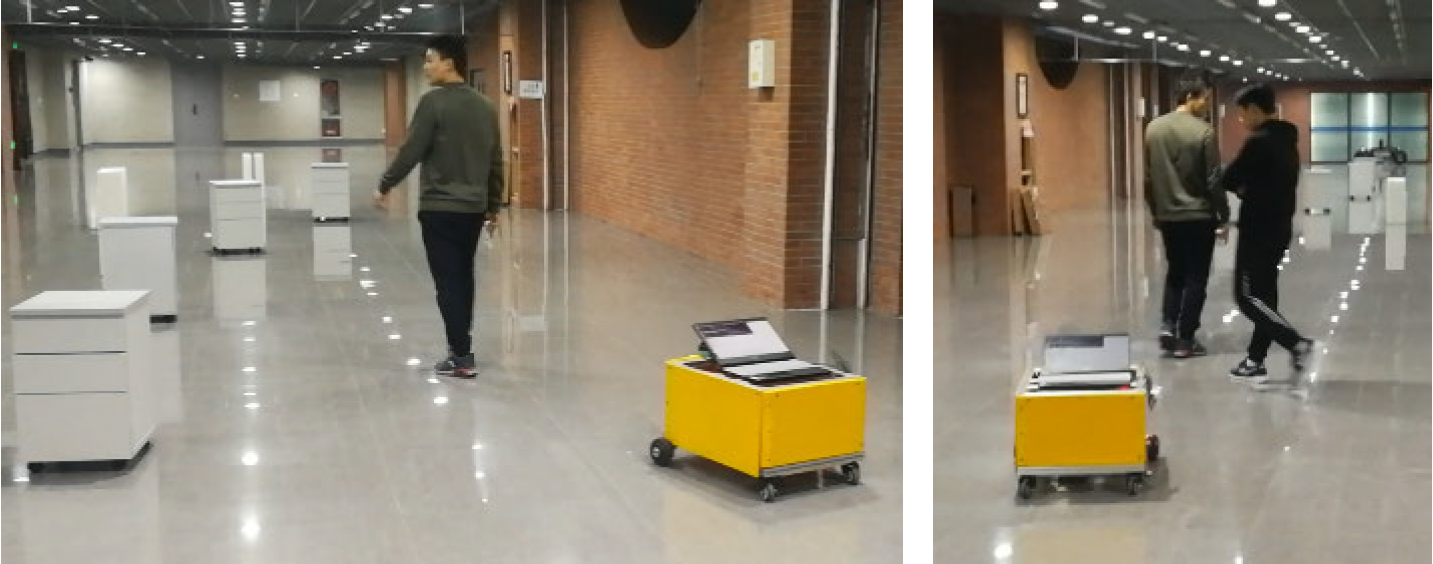
\includegraphics[height=60mm,clip]{figure/2-3_real.png}
  \caption{Person following in environments with obstacles
  \cite{A Robust Autonomous Following Method for Mobile Robots in Dynamic Environments}}
  \label{2-3_real}
  \end{center}
\end{figure*}

\begin{figure*}[h]
  \begin{center}
  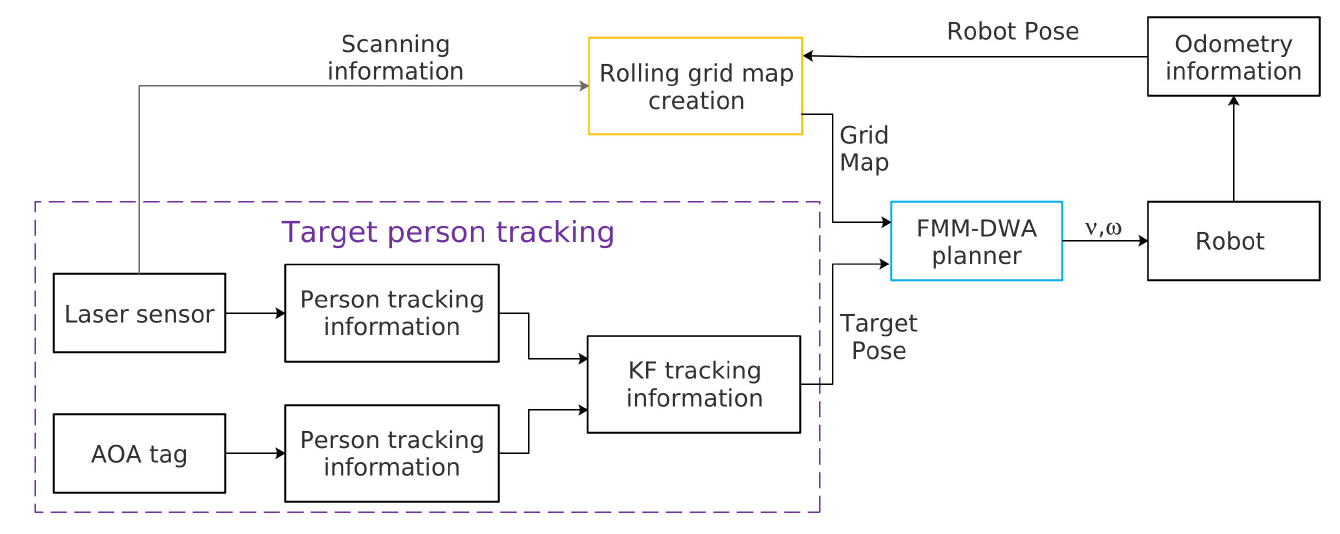
\includegraphics[height=60mm,clip]{figure/2-3_system.png}
  \caption{The architecture of our person-following system
  \cite{A Robust Autonomous Following Method for Mobile Robots in Dynamic Environments}}
  \label{2-3_system}
  \end{center}
\end{figure*}

\begin{figure*}[h]
  \begin{center}
  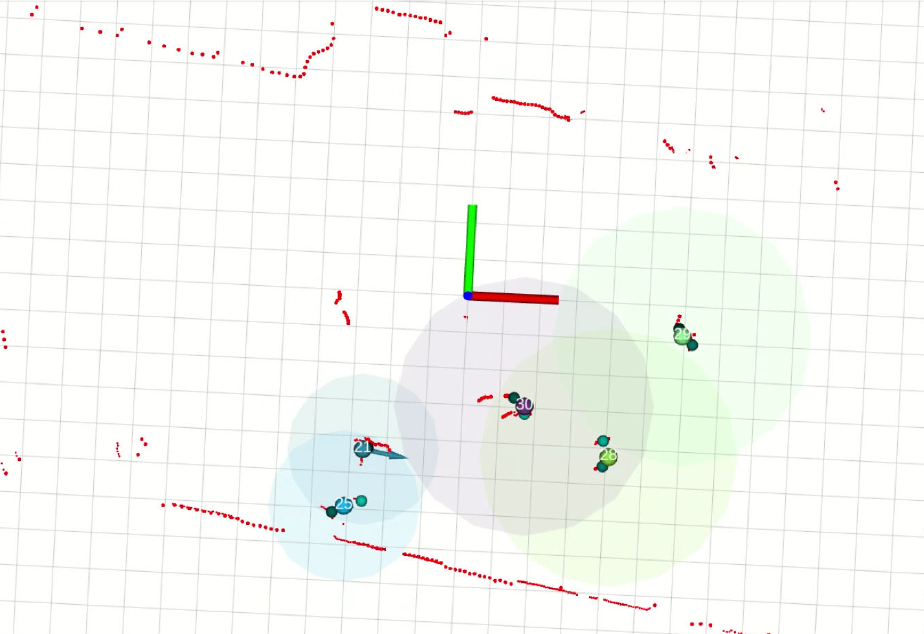
\includegraphics[height=70mm,clip]{figure/2-3_overview.png}
  \caption{Human legs detection and human tracking
  \cite{A Robust Autonomous Following Method for Mobile Robots in Dynamic Environments}}
  \label{2-3_overview}
  \end{center}
\end{figure*}

\begin{figure*}[h]
  \begin{center}
  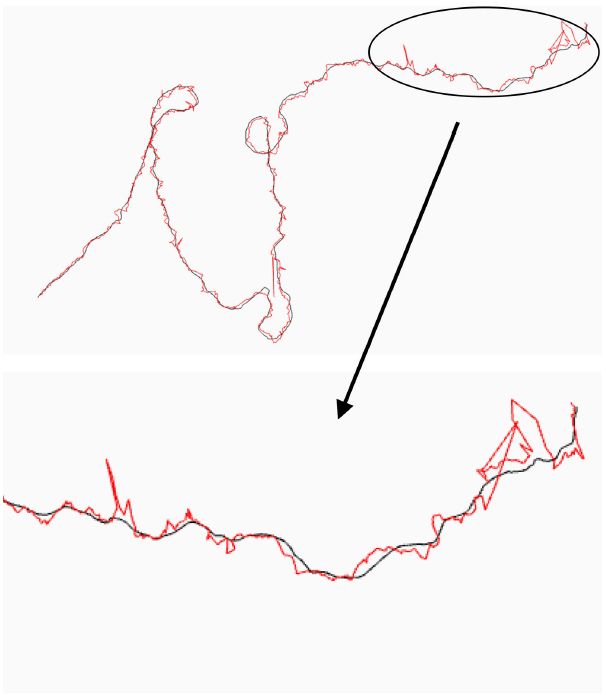
\includegraphics[height=110mm,clip]{figure/2-3_aoa.png}
  \caption{AOA tracking trajectory and Kalman filter trajectory
  \cite{A Robust Autonomous Following Method for Mobile Robots in Dynamic Environments}}
  \label{2-3_aoa}
  \end{center}
\end{figure*}

\begin{figure*}[h]
  \begin{center}
  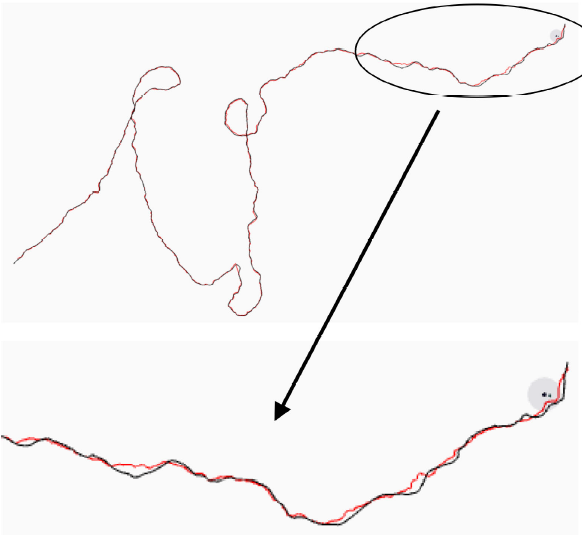
\includegraphics[height=100mm,clip]{figure/2-3_laser.png}
  \caption{Laser tracking trajectory and Kalman filter trajector
  \cite{A Robust Autonomous Following Method for Mobile Robots in Dynamic Environments}}
  \label{2-3_laser}
  \end{center}
\end{figure*}

\begin{figure*}[h]
  \begin{center}
  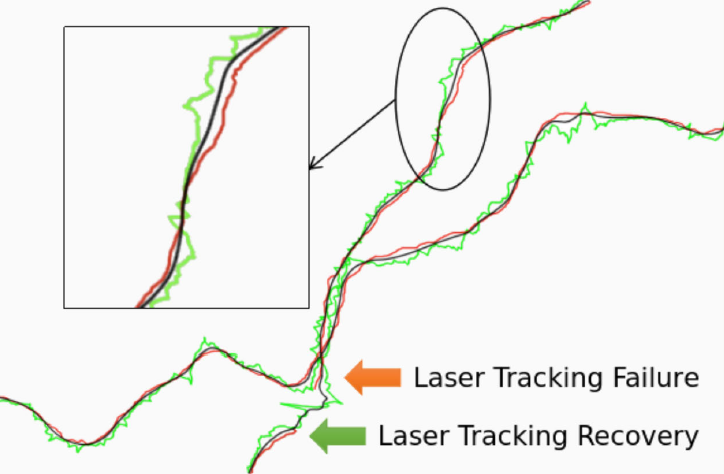
\includegraphics[height=70mm,clip]{figure/2-3_aoaANDlaser.png}
  \caption{Kalman filter tracking in occluded environments
  \cite{A Robust Autonomous Following Method for Mobile Robots in Dynamic Environments}}
  \label{2-3_aoaANDlaser}
  \end{center}
\end{figure*}

\begin{figure*}[h]
  \begin{center}
  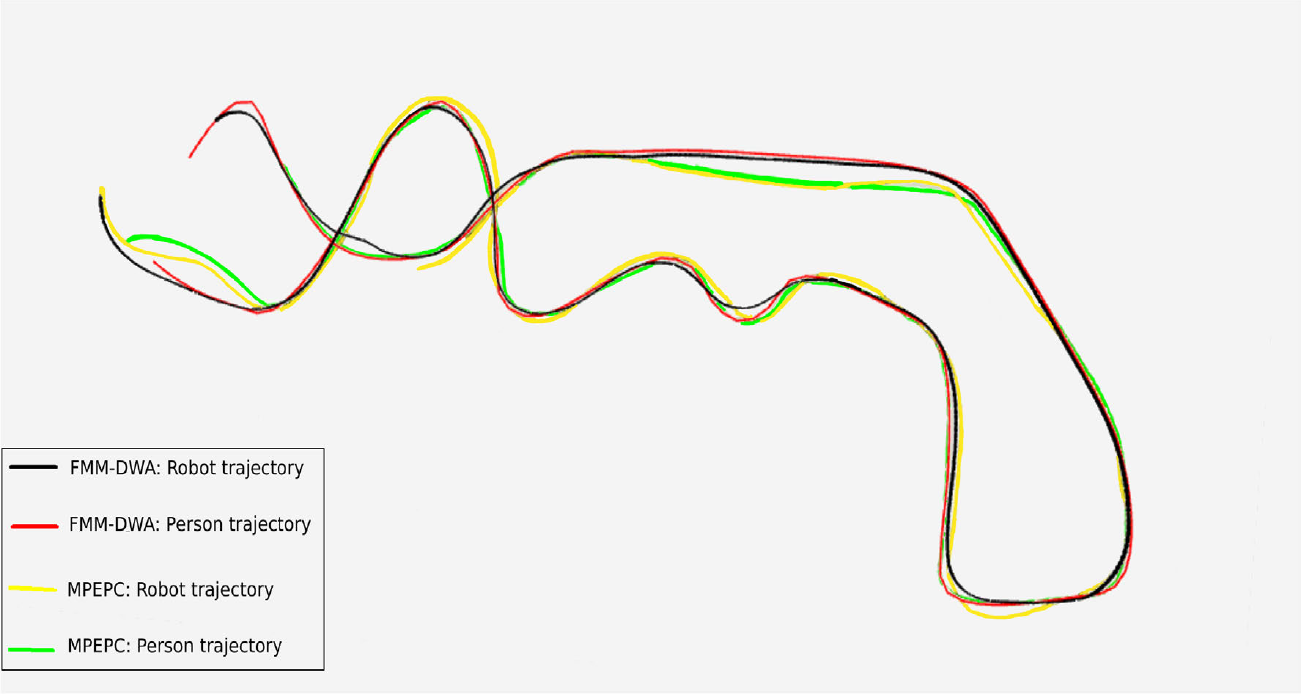
\includegraphics[height=70mm,clip]{figure/2-3_result.png}
  \caption{Following trajectory in environments with obstacles
  \cite{A Robust Autonomous Following Method for Mobile Robots in Dynamic Environments}}
  \label{2-3_result}
  \end{center}
\end{figure*}

\begin{table}[h]
  \begin{center}
    \caption{{Comparison of performance between FMM-DWA algorithm and MPEPC algorithm
    \cite{A Robust Autonomous Following Method for Mobile Robots in Dynamic Environments}}
    \label{2-3_result_table}}
    \scalebox{1.1}[0.9]{
      \begin{tabular}{c|c|c|c} \hline
        Method & $\alpha > 1$ & $r < 1$ & $S_r / S_h$ \\ \hline
        FMM-DWA & 8\% & 3\% & 94\% \\ \hline
        MPEPC & 32\% & 8\% & 95\% \\ \hline
      \end{tabular}
    }
  \end{center}
\end{table}

\clearpage

\section{従来研究における課題と本プロジェクトの位置づけ}
従来研究の課題として、2D-LiDARとYOLOv5を用いた手法では、雑多な環境下において人追従中に
周囲の環境に影響され、特定の追従目標を追従できない点が挙げられる。また、検出範囲が固定
であることから、人間がロボットの検出範囲に合わせながら歩行しなければならず、
人の歩行速度の低下に伴いロボットの追従速度も低下している点が課題として挙げられる。\\ \indent
2D-LiDARの距離データをクラスタリングする手法では、
人の脚部が幾何学的特徴からの検出であり、脚部に類似している物体が乱雑に配置されていた場合、
人の脚部ではない物体が誤検出されてしまう課題が考えられる。\\ \indent
FCNと2D-LiDARを用いた手法とAOAタグと2D-LiDARを用いた手法では、
物体が少ない綺麗な環境下での実験はされていないため、雑多な環境下での追従性能が不明である。
また、AOAタグと2D-LiDARを用いた手法では、人の脚部を幾何学的特徴を用いて検出しているため、
雑多な環境下での追従性能の低下やAOAタグの紛失などの課題が考えれる。
本プロジェクトでは、雑多な環境下において特定の人を追従し、
ロボットの最大直進速度で追従し続けらるような人追従システムを提案する。